% CSULA M.S. thesis format, modeled on the chair's sample thesis (Kuko).
% Generated by build_from_paper.py from ../paper/main.tex. Do not edit main.tex by hand.
\documentclass[12pt,oneside]{report}
\input{glyphtounicode}
\pdfgentounicode=1
\usepackage{cmap}
\usepackage[T1]{fontenc}
\usepackage[utf8]{inputenc}
\usepackage{lmodern}      % typewriter text (code identifiers)
\usepackage{mathptmx}     % Times roman body text, as in the sample (Times New Roman 12 pt)
% Sample: Letter, 1.25 in left/right, 1 in top/bottom, page number centered 0.5 in from bottom.
\usepackage[letterpaper,left=1.25in,right=1.25in,top=1in,bottom=1in,footskip=0.5in]{geometry}
\usepackage{setspace}
\usepackage{graphicx}
\usepackage{booktabs}
\usepackage{tabularx}
\usepackage{multirow}
\usepackage{array}
\usepackage{amsmath,amssymb}
\usepackage{xcolor}
\usepackage{tikz}
\usetikzlibrary{arrows.meta,positioning,fit,calc}
\usepackage{caption}
\usepackage{url}
\usepackage[numbers,sort&compress]{natbib}
\usepackage[expansion=false]{microtype}
\usepackage{xspace}
\usepackage{float}
\usepackage{multicol}
\usepackage{enumitem}
\usepackage{ragged2e}
\usepackage{titlesec}
\usepackage[titles]{tocloft}
\usepackage{chngcntr}
\usepackage{etoolbox}
\usepackage{needspace}
\usepackage[defaultlines=2,all]{nowidow}
% Floats single spaced (body stays double spaced); table rows padded like the sample's tables.
\AtBeginEnvironment{figure}{\singlespacing}
\AtBeginEnvironment{table}{\singlespacing\renewcommand{\arraystretch}{1.3}}
\usepackage{indentfirst} % sample indents the first paragraph of every chapter
\usepackage[hidelinks]{hyperref}

\graphicspath{{../paper/figures/}}

\hypersetup{
  pdftitle={State, Not Syntax: Harness Optimization for Small-Model Multi-Turn Tool Calling},
  pdfauthor={Sanskar Thapa}
}

\newcommand{\pp}{\,pp\xspace}
\newcommand{\placeholder}[1]{{\sloppy\textbf{[PLACEHOLDER: #1]}\par}}
\newcommand{\placeholderinline}[1]{\textbf{[PLACEHOLDER: #1]}}

% == Body: Word "double" spacing as in the sample (baseline pitch about 27.6 pt), ragged right,
%    0.5 in paragraph indent (sample "Research Style") ==
\newcommand{\thesisspacing}{\setstretch{1.91}}
\thesisspacing
\setlength{\parindent}{0.5in}
\setlength{\RaggedRightParindent}{0.5in}
\setlength{\RaggedRightRightskip}{0pt plus 1fil}
\hyphenpenalty=10000 % no hyphenation, as in the sample
\widowpenalty=10000
\clubpenalty=10000
\AtBeginDocument{\RaggedRight}
\setlength{\parskip}{0pt}
\setlength{\bibsep}{0pt}

% == Continuous figure/table numbering (sample: Table 1..6, Fig. 1..10) ==
\counterwithout{figure}{chapter}
\counterwithout{table}{chapter}

% == Captions: figures below as "Fig. N." (italic label), tables above as "TABLE N." ==
\captionsetup{font={small,singlespacing},labelsep=period,justification=raggedright,singlelinecheck=true}
\captionsetup[figure]{name={Fig.},labelfont=it}
\captionsetup[table]{name={Table},labelfont=sc,textfont=sc}
\renewcommand{\tablename}{Table}
\DeclareCaptionLabelFormat{tableup}{\MakeUppercase{#1}~#2}
\captionsetup[table]{labelformat=tableup,labelfont=up,textfont=sc,justification=centering}
\setlength{\abovecaptionskip}{4pt}
\setlength{\belowcaptionskip}{4pt}
\setlength{\intextsep}{12pt plus 2pt minus 2pt}

% == Headings (sample "Heading 1"): CHAPTER N / Title centered bold at top of a new page;
%      level-2 headings flush left bold, unnumbered. ==
\setcounter{secnumdepth}{0}  % number chapters only
\titleformat{\chapter}[display]{\normalfont\normalsize\bfseries\centering}{\MakeUppercase{\chaptertitlename}~\thechapter}{0pt}{}
\titlespacing*{\chapter}{0pt}{-\baselineskip}{\baselineskip}
\titleformat{name=\chapter,numberless}[block]{\normalfont\normalsize\centering}{}{0pt}{}
\titlespacing*{name=\chapter,numberless}{0pt}{-\baselineskip}{\baselineskip}
\titleformat{\section}[block]{\normalfont\normalsize\bfseries}{}{0pt}{}
\titlespacing*{\section}{0pt}{0pt}{0pt}
\titleformat{\subsection}[block]{\normalfont\normalsize\bfseries\itshape}{}{0pt}{}
\titlespacing*{\subsection}{0pt}{0pt}{0pt}
% unnumbered level-2 headings still go in the TOC (sample lists them)
\setcounter{tocdepth}{1}
\makeatletter
\let\orig@section\section
\renewcommand{\section}{\@ifstar{\orig@section*}{\thesis@sec}}
\newcommand{\thesis@sec}[1]{\Needspace{4\baselineskip}\orig@section*{#1}\phantomsection\addcontentsline{toc}{section}{#1}}
\makeatother

% == TOC / LOT / LOF in the sample's layout ==
\renewcommand{\contentsname}{TABLE OF CONTENTS}
\renewcommand{\listtablename}{LIST OF TABLES}
\renewcommand{\listfigurename}{LIST OF FIGURES}
\renewcommand{\cfttoctitlefont}{\hfill\normalfont\normalsize}
\renewcommand{\cftaftertoctitle}{\hfill}
\renewcommand{\cftlottitlefont}{\hfill\normalfont\normalsize}
\renewcommand{\cftafterlottitle}{\hfill}
\renewcommand{\cftloftitlefont}{\hfill\normalfont\normalsize}
\renewcommand{\cftafterloftitle}{\hfill}
\setlength{\cftbeforetoctitleskip}{-\baselineskip}
\setlength{\cftbeforelottitleskip}{-\baselineskip}
\setlength{\cftbeforeloftitleskip}{-\baselineskip}
\setlength{\cftaftertoctitleskip}{\baselineskip}
\setlength{\cftafterlottitleskip}{\baselineskip}
\setlength{\cftafterloftitleskip}{\baselineskip}
% front/back-matter entries (Abstract, ..., References, Appendices): flush left, dotted
\renewcommand{\cftpartfont}{\normalfont}
\renewcommand{\cftpartpagefont}{\normalfont}
\renewcommand{\cftpartleader}{\cftdotfill{\cftdotsep}}
\setlength{\cftbeforepartskip}{0pt}
\setlength{\cftpartindent}{0pt}
% chapters: "1. Introduction", indented 0.5 in, dotted, not bold
\renewcommand{\cftchapfont}{\normalfont}
\renewcommand{\cftchappagefont}{\normalfont}
\renewcommand{\cftchapleader}{\cftdotfill{\cftdotsep}}
\renewcommand{\cftchapaftersnum}{.}
\setlength{\cftbeforechapskip}{0pt}
\setlength{\cftchapindent}{0.5in}
\setlength{\cftchapnumwidth}{2em}
% level-2 headings: indented 1.0 in
\setlength{\cftsecindent}{1.0in}
\setlength{\cftsecnumwidth}{0pt}
% list entries: "1. caption", indented
\renewcommand{\cftfigaftersnum}{.}
\renewcommand{\cfttabaftersnum}{.}
\setlength{\cftfigindent}{0.25in}
\setlength{\cfttabindent}{0.25in}
\setlength{\cftfignumwidth}{2.2em}
\setlength{\cfttabnumwidth}{2.2em}
\setlength{\cftbeforefigskip}{4pt}
\setlength{\cftbeforetabskip}{4pt}
\cftsetrmarg{3.2em plus 1fil}
\cftsetpnumwidth{2em}
\renewcommand{\cftdotsep}{1}
% Leaders always get at least 2 em, so an entry whose text fills its last line moves its
% last word down instead of printing the page number with no dots.
\makeatletter
\renewcommand{\cftdotfill}[1]{\leaders\hbox{$\m@th\mkern #1 mu\hbox{\cftdot}\mkern #1 mu$}\hskip 2em plus 1fill}
\makeatother
\newcommand{\tocline}[1]{\phantomsection\addcontentsline{toc}{part}{#1}}
\pdfstringdefDisableCommands{\def\pp{ pp}}

% Keep floats close to their paragraph.
\renewcommand{\topfraction}{0.85}
\renewcommand{\bottomfraction}{0.8}
\renewcommand{\textfraction}{0.1}
\renewcommand{\floatpagefraction}{0.7}

\begin{document}

%======================== FRONT MATTER (lower-case roman) ========================
\pagenumbering{roman}

% == Title page (page i, number not printed) ==
\begin{titlepage}
\centering\thesisspacing
STATE, NOT SYNTAX: HARNESS OPTIMIZATION FOR\\
SMALL-MODEL MULTI-TURN TOOL CALLING

\vfill
A Thesis\\
Presented to\\
The Faculty of the Department of Computer Science\\
California State University, Los Angeles

\vfill
In Partial Fulfillment\\
of the Requirements for the Degree\\
Master of Science\\
in\\
Computer Science

\vfill
By\\
Sanskar Thapa\\
December 2026
\end{titlepage}

% == Copyright page (ii) ==
\setcounter{page}{2}
\thispagestyle{plain}
\null\vfill
\begin{center}\singlespacing
\copyright{} 2026\\[\baselineskip]
Sanskar Thapa\\[\baselineskip]
ALL RIGHTS RESERVED
\end{center}
\clearpage

% == Approval / committee page (iii) ==
\thispagestyle{plain}
\begin{center}
The thesis of Sanskar Thapa is approved.

Dr. Mohammad Pourhomayoun, Committee Chair

\placeholderinline{Committee member name}

\placeholderinline{Committee member name}

Dr. Chengyu Sun, Department Chair

\vspace{3\baselineskip}
California State University, Los Angeles

December 2026
\end{center}
\clearpage

% == Abstract (iv) ==
\chapter*{ABSTRACT}
\vspace{-\baselineskip}% title block directly under the heading, as in the sample
\tocline{Abstract}
{\centering
State, Not Syntax: Harness Optimization for\\
Small-Model Multi-Turn Tool Calling\\
By\\
Sanskar Thapa\par}

Small language models can run on a laptop and call tools to act for a user, but they often fail when a task needs several calls in a row. This thesis asks why, and what helps, using Gemma-4-E2B-it, a model with about two billion effective parameters, on 200 multi-turn tasks from the Berkeley Function Calling Leaderboard. Tasks are graded by the final state of a simulated backend, for example whether a car's engine is on.

The main finding is that the model fails at deciding what to do next, not at writing calls. It handles single calls well (91.9\%) but completes only 27.0\% of multi-turn tasks, and forcing every call to be valid syntax made results worse. The remedy is a harness, the program around the model, with the weights untouched. It records the current state for the model, stops repeated calls, and adds a short card advising whether to call, ask, finish or refuse. This raised accuracy from 30.5\% to 38.5\%, a suggestive gain, and matched a five-sample vote at about a seventh of the generation time. Writing the tool list more compactly added about 7 points in two paired runs, the best reaching 44.0\%. Wrong final states remain the largest failure type. Fine-tuning the model did not help; the best tuned model scored 15.0\%, below the untuned model.


% == Acknowledgments: left out until Sanskar writes them. ==
% Uncomment the three lines below to restore the page and its table-of-contents entry.
%\chapter*{ACKNOWLEDGMENTS}
%\tocline{Acknowledgments}
%\placeholder{Acknowledgments, to be written by Sanskar}
\clearpage

% == Table of contents, lists ==
\begingroup
\renewcommand{\cftpartfont}{\normalfont}
\tableofcontents
\endgroup
\clearpage
\tocline{List of Tables}
\begingroup\singlespacing\hyphenpenalty=10000
\renewcommand{\addvspace}[1]{}% drop the per-chapter 10 pt gaps so entry spacing is even
\listoftables
\endgroup
\vspace{\baselineskip}
\tocline{List of Figures}
\begingroup\singlespacing\hyphenpenalty=10000
\renewcommand{\addvspace}[1]{}% drop the per-chapter 10 pt gaps so entry spacing is even
\let\clearpage\relax
\let\cleardoublepage\relax
\listoffigures
\endgroup
\addtocontents{lot}{\protect\noindent Table\protect\par}
\addtocontents{lof}{\protect\noindent Figure\protect\par}

% Glossary follows the lists on the same page so a short list does not sit alone.
% Acknowledgments stay commented out above; this does not reorder title, copyright,
% approval, abstract, or the three lists.
\vspace{\baselineskip}
\begin{center}
GLOSSARY
\end{center}
\tocline{Glossary}
\begingroup\singlespacing
\setlength{\multicolsep}{0pt}
\begin{multicols}{2}\scriptsize
\begin{description}[leftmargin=0pt,itemsep=0pt,parsep=0pt,topsep=0pt]
\item[AST] Abstract syntax tree; the single-turn BFCL matcher.
\item[BFCL] Berkeley Function Calling Leaderboard.
\item[DPO] Direct Preference Optimization.
\item[Full stack] JSON text + state summary + stop on repeats + status card.
\item[Greedy decoding] Always picking the most likely next token (temperature 0). Repeat runs can still differ.
\item[Harness] The program around the model that parses calls, runs tools and records state.
\item[JSON text] Calls written as a JSON list in ordinary text, which the harness parses. Logs abbreviate this IFFC.
\item[LoRA] Low-rank adapters: small trainable matrices added to frozen weights.
\item[McNemar test] A paired test using only tasks where two conditions disagree.
\item[Minimal recipe] JSON text + stop on repeats + status card.
\item[Native API] Structured \texttt{tool\_calls} from the server's tool interface. Logs abbreviate this NFC.
\item[Null test] A training run that should change nothing if the pipeline is sound.
\item[OODA] Observe--orient--decide--act; here only the tag printed on the status card.
\item[pp] Percentage points.
\item[Q4\_K\_M] A 4-bit weight-quantization format of llama.cpp.
\item[Self-distillation] Training the model on its own answers to simulated tasks that a checker marked correct.
\item[SFT] Supervised fine-tuning.
\item[Sign test] A paired test counting the tasks on which one condition solved more of its runs than the other; tasks with equal counts are dropped.
\item[Slot] One request a server processes concurrently with others.
\item[State summary] Harness-written snapshot of facts from executed results.
\item[Status card] Four-line card prefixed to the latest user message.
\item[Stop on repeats] Ends a turn when the model re-proposes executed calls.
\item[Stop target] A training response that is an empty list: no further call.
\item[Tool-name automaton] Program that constrains only the tool name.
\item[Turn] One user request and everything the model does before handing control back.
\item[Vote of five] Majority vote over five sampled calls per step.
\item[Wilson interval] A confidence interval for a proportion that stays accurate for small counts.
\item[20-task gate] Fixed 20-task screening check (bar 17/20); not a 200-task accuracy.
\end{description}
\end{multicols}
\endgroup
\clearpage
\addtocontents{toc}{\protect\noindent Chapter\protect\par}

%======================== BODY (arabic, from 1) ========================
\clearpage
\pagenumbering{arabic}

\chapter{Introduction}
\label{sec:intro}

To check a calendar or lock a car, a language model emits a \emph{tool call}: a function name plus arguments. A surrounding program, the \emph{harness}, runs the call against a \emph{backend} (here a simulated vehicle or filesystem) and feeds the result back to the model (Figure~\ref{fig:vignette}). Real tasks chain several dependent calls, which we call \emph{multi-turn} tool calling: look up a value, use it, check the outcome, and know when to stop.

\begin{figure}[H]
\centering
\begin{tikzpicture}[
  font=\footnotesize,
  box/.style={draw, rounded corners=2pt, align=left, inner sep=3pt, fill=gray!5, text width=0.86\textwidth},
  arr/.style={-{Latex}, thick}
]
\node[box] (user) {\textbf{User.} ``Lock the doors and start the engine.''};
\node[box, below=0.16cm of user] (s1) {\textbf{Model} emits \texttt{lockDoors()} (as JSON text, or in a native \texttt{tool\_calls} field). \textbf{Harness} runs it on the simulated vehicle and returns \texttt{\{"lockStatus": "locked"\}}.};
\node[box, below=0.16cm of s1] (s2) {\textbf{Model} emits \texttt{startEngine()}. \textbf{Harness} returns an error: the brake pedal must be pressed first.};
\node[box, below=0.16cm of s2] (chk) {\textbf{Checker} compares the vehicle's \emph{final state} with a reference. Typical failure: every call was valid JSON, but the model never pressed the brake and retried, so the engine is off and the final state is wrong.};
\draw[arr] (user) -- (s1); \draw[arr] (s1) -- (s2); \draw[arr] (s2) -- (chk);
\end{tikzpicture}
\caption[The multi-turn tool-calling loop]{The multi-turn tool-calling loop studied in this thesis. Grading uses the final state of the simulated backend; whether the calls parse is not enough. Illustrative, not a scored task.}
\label{fig:vignette}
\end{figure}

Running this loop locally with a small model keeps private data on the device, works offline and has no per-request cost. The catch is accuracy. We study Gemma-4-E2B-it~\cite{gemma4e2b} (``E2B'': about two billion effective parameters, meaning the inference footprint; ``it'': instruction-tuned) on BFCL v4~\cite{patil2024bfcl}, served with the llama.cpp inference engine~\cite{llamacpp} on a laptop. Through the server's built-in tool-call field, the native API, it completes 27.0\% of 200 multi-turn tasks.

Is the model failing to \emph{write} calls or to \emph{choose} them? Chapter~\ref{sec:fail} shows it is mostly the latter: tasks fail because a needed tool never ran or the backend ended in the wrong state. We therefore treat the problem as \emph{harness optimization}. The weights stay fixed; we change the loop around the model: how calls are parsed, what state the harness records and shows back, when it ends a turn, and how the next step is framed. Two of these levers, a state summary and a status card, reach the model as text in its context, so the harness acts partly through the context; both are computed from executed results. We compare harness control with two other families of fixes: forcing syntactically valid output, and fine-tuning the weights. Our contributions:

\begin{enumerate}
  \item \textbf{Where the failures are.} The model usually handles a single call, and it usually fails when the task needs several. A needed call never happens, or the backend ends in the wrong state. Forcing each call to be valid syntax makes this worse (Chapter~\ref{sec:fail}).
  \item \textbf{A harness that helps without training.} The weights stay fixed. The program around the model records the current state, stops repeated calls, and shows a short card advising the next move. Together these raise accuracy by a suggestive amount. A more compact tool list helps further, and the harness keeps up with a five-sample vote at a fraction of the generation time (Chapter~\ref{sec:helps}).
  \item \textbf{Fine-tuning did not help.} The best supervised fine-tune scores below the untuned model, and preference tuning does not beat it. A control fine-tune that should change nothing, if the machinery is sound, stays close to the untuned model. The later training set is the leading suspect, and it also differed in training length (Chapter~\ref{sec:train}).
\end{enumerate}

The rest of this thesis is organized as follows. Chapters~\ref{sec:related} to~\ref{sec:fail} introduce the benchmark, the setup, and the failures. Chapters~\ref{sec:helps} and~\ref{sec:train} report the harness and the fine-tuning. Chapter~\ref{sec:discussion} says what to use, Chapter~\ref{sec:conclusion} closes with future work and the conclusion, and the appendices hold the details and the full list of runs.

\chapter{Background and Related Work}
\label{sec:related}

This chapter names the benchmark and the ideas the experiments rely on: how a call is written, what it means to force that writing to be valid, what the program around the model can do, and how training a tool-calling model is usually done.

\section{Benchmark}

The Berkeley Function Calling Leaderboard (BFCL) evaluates language models as API callers~\cite{patil2023gorilla,patil2024bfcl}. Its single-turn categories check one emitted call against a reference with an abstract-syntax-tree (AST) matcher. Its multi-turn categories run the model in an agent loop against simulated backends (for example VehicleControl and GorillaFileSystem, a sandboxed Unix-like filesystem) and compare the backends' final state with a reference. A \emph{turn} is one user request and everything the model does before handing control back; each multi-turn task has several turns. We use the \emph{multi-turn base} split (200 tasks, all tools available). Accuracy is the fraction of the 200 tasks whose final state matches.

\section{Output Channel}

With the \emph{native API}, the server receives a tool list and the model returns structured \texttt{tool\_calls}, as in most production APIs. With \emph{JSON text}, the prompt asks the model to write its calls as a JSON list in ordinary text, which the harness parses. Taheri et al.\ report that small models follow such JSON instructions more reliably than native tool APIs on single-turn BFCL~\cite{taheri2026iffc}; we use their single-model variant.

\section{Constrained Decoding}

Grammar-constrained generation restricts each next token so that output is always valid, for example to a JSON schema or a list of tool names~\cite{willard2023outlines,dong2026xgrammar2}; Yu et al.\ constrain tool names with a token-level automaton~\cite{yu2026ptc}. Format restrictions can also reduce answer quality~\cite{tam2024format}. Chapter~\ref{sec:fail} tests whether forcing validity helps in a multi-turn loop.

\section{Harness-Side Control and Test-Time Compute}

Context-compression methods summarize long histories~\cite{kang2025acon}; our state summary is instead written by the harness from executed results. Observe--orient--decide--act (OODA) controllers structure agent steps~\cite{guo2026ooda}; our status card borrows only the name. Guided templates add a reasoning scaffold before calls~\cite{he2025gst}. Sampling several answers and voting is a standard way to buy accuracy with compute~\cite{snell2024testtime}; our vote of five is that baseline.

\section{Training for Tool Use}

Specialist small callers such as xLAM~\cite{zhang2024xlam} and Hammer~\cite{ye2025hammer} are trained on synthetic tool data such as ToolACE~\cite{liu2024toolace} and APIGen~\cite{liu2024apigen}. \emph{Supervised fine-tuning} (SFT) trains the model to reproduce target responses; we use low-rank adapters (LoRA)~\cite{hu2021lora}, small trainable matrices added to frozen weights. \emph{Direct Preference Optimization} (DPO) trains on pairs of preferred and rejected responses~\cite{rafailov2023dpo,jung2025diatool}. Terms used in this thesis are collected in the glossary before Chapter 1.

The following chapters use only these ideas. They ask where a small model fails, whether the harness can help with the weights left fixed, and whether fine-tuning can.


\chapter{Setup and Methods}
\label{sec:setup}

\section{Model and Serving}

All results use Gemma-4-E2B-it, quantized with Q4\_K\_M (a 4-bit weight format of llama.cpp), served by \texttt{llama-server} on a laptop. Decoding is greedy (temperature 0) except for majority voting. Greedy runs are not identical from one run to the next (Chapter~\ref{sec:helps}). The machine, the server build, and the flags are in Appendix~\ref{app:runs}. Most runs used four parallel server slots (requests the server processes at the same time) and the native API baseline used eight, a serving difference that could affect its results. This thesis did not test whether the eight-slot and four-slot greedy outputs match.


\section{Harness Interventions}

All leave the weights untouched. A task is correct only when the BFCL multi-turn checker returns valid. Appendix~\ref{app:method} gives the rule for each intervention except the shorter tool list. By design, the state summary targets lost state, the stop rule targets runaway repetition, and the status card targets the choice between acting and abstaining.
\begin{itemize}\setlength{\itemsep}{1pt}
  \item \textbf{JSON text} instead of the native API. The harness parses the calls.
  \item \textbf{State summary.} After each executed call, the harness writes a short \texttt{[STATE]} snapshot of facts from real results (current directory, known files, last calls) into the conversation.
  \item \textbf{Stop on repeats.} The harness ends the current turn when the model repeats its previous set of calls, or when it re-proposes calls already executed in this turn after at least six tool steps. An \emph{ungated} variant drops the six-step minimum.
  \item \textbf{Status card.} A four-line card (goal, known facts, last call and outcome, and an advisory next move: call, ask, finish, or refuse) is prefixed to the latest user message. The card prints finish as \texttt{final}. The harness fills the card from fixed rules on the conversation and executed results; it never sees reference answers. JSON text, stop on repeats, and the card, together, are the \emph{minimal recipe}.
  \item \textbf{Full stack.} JSON text, the state summary, stop on repeats, and the status card, decoded greedily. On its first run this is the harness we compare with JSON text.
  \item \textbf{Shorter tool list.} On the full stack, every tool stays in the prompt. The harness states each tool group's shared description once, instead of repeating it, and prints each schema without indentation. The model, the four pieces above, and the tasks stay the same. The shorter list is text in the context, so this lever, like the state summary and the status card, is harness-side control delivered through the context.
  \item \textbf{Vote of five.} On top of the state summary, at each step the harness samples five candidate calls at temperature 0.7 and executes the most common one. This is the compute-heavy comparison point.
  \item \textbf{Forced-valid decoding.} \emph{Constrained decoding} restricts output in two passes (tool names, then arguments by schema). A \emph{tool-name automaton} constrains only the name, inspired by~\cite{yu2026ptc}.
\end{itemize}

The state summary and the status card are short notes the harness writes from results it has already executed. A state summary looks like this:
\begin{quote}\singlespacing\footnotesize\ttfamily
[STATE]\\ cwd: /workspace/notes\\ files: todo.txt, log.csv\\ last: cd(folder='notes')->ok
\end{quote}
A status card, prefixed to the latest user message, looks like this:
\begin{quote}\singlespacing\footnotesize\ttfamily
[OODA]\\ goal: lock the doors and start the engine\\ slots: lockStatus=locked\\ last: startEngine()->error: brake pedal must be pressed\\ next: call
\end{quote}


\section{Training}

We train LoRA adapters on Gemma-4-E2B-it with MLX~\cite{mlx}, Apple's machine-learning framework, merge them into the weights, quantize to Q4\_K\_M and evaluate with JSON text. Early mixes combine ToolACE dialogues with sampled xLAM data; a later \emph{rebuilt mix} (30{,}000 rows) combines about 45\% newly simulated, execution-checked episodes with cleaned public data. We also train one DPO model. Because full 200-task runs are slow, trained models first face a fixed 20-task \emph{gate} drawn from the same split and run with the status card; the bar is 17/20, the untuned model's score with the card.

\section{Error Labels}

Each failed task gets one primary label from the checker's message: \emph{empty turn} (no call on a turn that needed one), \emph{under-call} (a required tool never ran), or \emph{state mismatch} (tools ran but the backend's final state differs from the reference). Output the harness cannot parse counts as no call, so a parse failure can only appear as an empty turn.

\section{Statistics}

Each reported accuracy comes with a Wilson 95\% interval~\cite{wilson1927}, a range that stays reliable when few tasks are correct. When two conditions are compared on the same 200 tasks, we use an exact two-sided McNemar test~\cite{mcnemar1947}. It counts only the tasks the two conditions decide differently. The $p$-value is the chance of a gap at least that large if the conditions were equal.

Eight comparisons were planned as one family. The family covers the full stack and the minimal recipe against their baselines, the switch from the native API to JSON text, and the best fine-tune. Four of the eight use the full stack, and the family was fixed after that configuration was built. Four single-lever comparisons are exploratory and were left out of the family (Table~\ref{tab:mcnemar-x}): the state summary against JSON text, the vote against the state summary, stop on repeats against JSON text, and the minimal recipe against stop on repeats. We report the raw $p$-value, and we say when Holm's correction~\cite{holm1979} changes the conclusion. That correction keeps the chance of any false alarm among the eight tests at 5\%.

The shorter tool list is not one of the eight tests. It is judged at the 0.05 level set in the plan. It was run as two pairs, the second in the opposite order. To combine them, we count how many of its two runs each list solved for each task, and we apply an exact two-sided sign test to the tasks where the counts differ. Why the comparison uses a fresh rerun, rather than the first full-stack run, is recorded in Appendix~\ref{app:trim}.



\chapter{Where Small Models Fail}
\label{sec:fail}

\section{One Call Is Easy; a Chain Is Not}

On three single-call BFCL categories (840 cases), Gemma-4-E2B-it through the native API scores 772/840 (91.9\%, interval 89.9--93.6\%; Table~\ref{tab:board}). \emph{Simple} offers one function and asks for that call (375/400). \emph{Multiple} offers several functions and asks for the right one (183/200). \emph{Irrelevance} offers functions when the query needs no call (214/240). The two parallel-call categories are excluded because earlier runs on this server hit a tool-grammar bug that truncated multi-call output. On multi-turn tasks, the \emph{same model, quantization and server} completes only 54 of 200 (27.0\%). The two settings differ in grading as well as length, but the gap is consistent with carrying a chain of calls through a changing state, rather than choosing one call, being the bottleneck.

\section{Most Failures Are About the World}

A \emph{state mismatch} is a task where the calls ran and the backend still ended wrong. The loop in Figure~\ref{fig:vignette} is an example. The model locks the doors and then tries to start the engine. Both calls are valid. The backend says the brake pedal has to be pressed first. The model never presses it, so the engine stays off and the check fails.

Figure~\ref{fig:fail} breaks down the failed tasks (full counts in Table~\ref{tab:failfull}). For every JSON-text condition, state mismatch is the largest bucket (53--109 tasks). With plain JSON text it is followed by empty turns (41) and under-calls (38); the native API has more empty turns (59) and far fewer under-calls (19). Harness control mainly removes empty turns: the full stack has 20, against 41 for JSON text, while its state mismatches are 68 (60 for JSON text). Because parse failures can only appear as empty turns, most of what remains is not a formatting problem.

\begin{figure}[H]
\centering
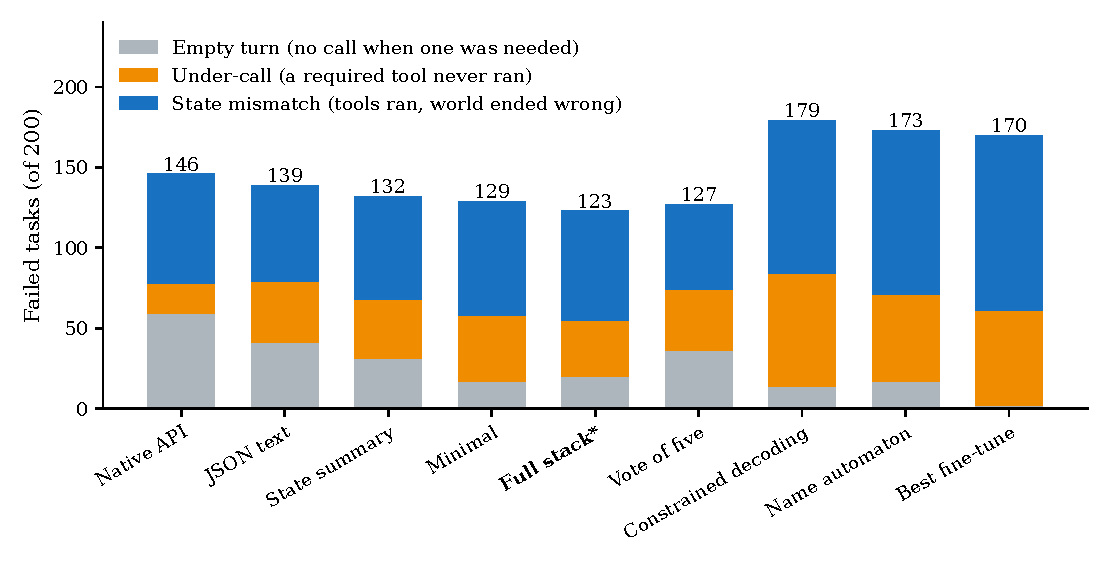
\includegraphics[width=\textwidth]{failure_anatomy.pdf}
\caption[Why multi-turn tasks fail]{Why tasks fail. Each bar is one condition on the same 200 tasks (* marks the first full-stack run; Constr.\ decod.\ = constrained decoding; Name autom.\ = tool-name automaton; Best SFT = best fine-tune; conditions as in Chapter~\ref{sec:setup}); its height is the number of failed tasks, split by primary error label (Chapter~\ref{sec:setup}). Harness control mostly removes empty turns (grey); wrong final states (blue) remain. Forced-valid output and the best fine-tune shift failures into under-calls (orange) and state mismatches. The shorter tool list is omitted.}
\label{fig:fail}
\end{figure}

\section{Forcing Valid Syntax Hurts}

If failures were mostly malformed output, guaranteeing valid output should help. It does the opposite. Two-pass constrained decoding scores 21/200 (10.5\%; interval 7.0--15.5\%), 20.0\pp below JSON text, with 70 under-calls and 95 state mismatches. The tool-name automaton scores 27/200 (13.5\%; 9.4--18.9\%), with state mismatch rising to 102. Our two-pass program, which forces each call into valid syntax, approximates rather than reproduces full grammar engines~\cite{dong2026xgrammar2}, but the effect is large and in the wrong direction: a valid call is not a correct next step.

\chapter{What Helps: Harness-Side Control}
\label{sec:helps}

If the bottleneck is choosing the next step, the harness, which sees every executed result, is a natural place to intervene. Every change below is greedy except the vote of five, and none touches the weights. Exact counts and intervals for every condition are in Table~\ref{tab:board} (Appendix~\ref{app:runs}).

\section{JSON Text over the Native API}

Writing calls as JSON text scores 61/200 against 54/200 on the native API, 3.5 percentage points higher ($p=0.32$, not significant). Part of the gap may come from serving. A seven-step reasoning template on the native API also scored 61/200, tying JSON text: 19 tasks swap each way, and state mismatches rose to 79. The gap may therefore reflect the shape of the prompt as much as which channel carries the call. We do not claim the channel switch alone as a gain. Later steps are built on JSON text because the harness can parse and inspect those calls directly. The harness levers were not tested on the native API, or combined with the template.


\section{State Summary}

The harness-written snapshot scores 68/200, 3.5 percentage points above JSON text ($p=0.30$). Empty turns fall from 41 to 31 while state mismatches do not (60 to 64), suggesting that the summary mainly keeps the model calling.

\section{Stop on Repeats and the Status Card}

The gated stop rule scores 65/200 (+2.0\pp, $p=0.48$). Stopping at the \emph{first} repeat instead scores 54/200, 11 tasks below the gated rule, and all 37 forced stops fell on tasks that failed. Adding the status card gives the minimal recipe, 71/200 (35.5\%, +5.0\pp over JSON text, $p=0.16$). Relative to stop on repeats alone, empty turns fall from 38 to 17 while state mismatches rise from 60 to 71, so the error labels suggest the card acts mainly as an act-versus-abstain control.

\section{Full Stack}

Combining all four greedy changes scores 77/200 (38.5\%, interval 32.0--45.4\%). Paired against JSON text, it solves 30 tasks that JSON text misses and misses 14 that JSON text solves (Table~\ref{tab:mcnemar}). Against the minimal recipe, the state summary alone, and the vote of five, the differences are within noise. The configuration was assembled after we had seen earlier results on these tasks, so its lead is subject to tuning leakage (Chapter~\ref{sec:discussion}).

\section{Shorter Tool List, Same Tools}

The full stack still sends every tool. The list is long because tools that share a group also share a description, and that description was repeated on every tool, with each schema indented. We state each group's shared description once and print the schemas without indentation. Nothing else changes: the model, the four pieces above, and the tasks stay the same. Like the state summary and the card, this reaches the model as text in its context.

We compared the shorter list with a fresh run of the original list, then repeated the comparison with the shorter list run first (Table~\ref{tab:trim}). The shorter list scores 84 of 200 (42.0\%) against 71 of 200 (35.5\%) in the first pair, and 88 of 200 (44.0\%) against 72 of 200 (36.0\%) in the second. The second pair is the best single run. The first pair falls just short of the 0.05 level set in the plan, and the second clears it. Counting each task once across both pairs, the shorter list does better on 33 tasks and the original list on 17, with 150 ties ($p=0.033$). The gain replicated. It is modest, about 7 points, and repeat runs still move individual tasks: the original list changed on 15 tasks and the shorter list on 18. Length and timing are in Appendix~\ref{app:trim}.

\begin{table}[H]
\centering
\footnotesize
\caption[Shorter tool list against the original list]{Shorter tool list against the original list (same model, tasks, and other harness parts). Pair 1 compares the shorter list with a fresh run of the original list. Pair 2 runs the shorter list first. ``Shorter only'' counts tasks the shorter list solves and the original list misses. $p$ is an exact two-sided McNemar test, judged at the 0.05 level set in the plan, outside Table~\ref{tab:mcnemar}.}
\label{tab:trim}
\begin{tabular}{@{}lrrrrc@{}}
\toprule
 & Shorter only & Original only & Both & Neither & $p$ \\
\midrule
Pair 1 & 26 & 13 & 58 & 103 & 0.053 \\
Pair 2 & 26 & 10 & 62 & 102 & 0.011 \\
\bottomrule
\end{tabular}
\end{table}

Figure~\ref{fig:ladder} shows these runs on one scale. The top bar is the shorter tool list.

\begin{figure}[H]
\centering
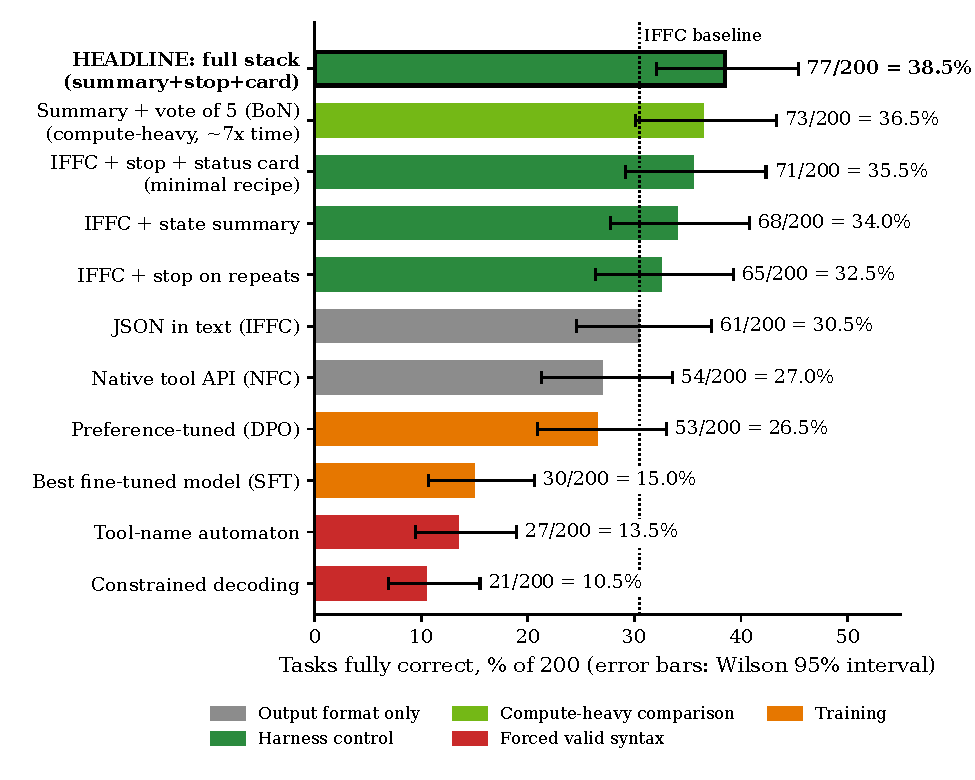
\includegraphics[width=\textwidth]{ladder_n200.pdf}
\caption[Multi-turn accuracy by condition]{Multi-turn accuracy on 200 BFCL v4 tasks, Gemma-4-E2B-it. Each bar is a separate run, not a stack of the bars below it. Bars: share of tasks fully correct; error bars: Wilson 95\% intervals. Dark green: harness control on JSON text (the first full-stack run is outlined and in bold); light green: majority vote, the compute-heavy comparison; grey: output format alone; red: forced-valid output; orange: training. Dotted line: JSON-text baseline (30.5\%). Top bar: the full stack with a shorter tool list, the better of its two runs (88/200; the other scored 84/200, and two reruns of the original list scored 71/200 and 72/200; Table~\ref{tab:trim}).}
\label{fig:ladder}
\end{figure}



\section{Majority Vote}

Voting over five samples on top of the state summary scores 73/200 (36.5\%), four tasks fewer than the first full-stack run, which solves 24 tasks the vote misses and misses 20 it solves ($p=0.65$). The vote takes about $7\times$ as long to generate as the greedy full stack, from a single sampling seed. A greedy harness matches it at a fraction of the time, which matters on a local device.

\section{How Sure Are We?}

Each harness accuracy comes with a range that extends about six to seven percentage points on either side (Table~\ref{tab:board}). A gap smaller than that can be noise. Of the eight planned comparisons (Table~\ref{tab:mcnemar}), two harness gaps fall below 0.05 on their own: the full stack against JSON text ($p=0.023$) and the minimal recipe against the native API ($p=0.033$). Neither stays below 0.05 after correcting for the eight tests. The order of the harness rows is therefore tentative, and the full stack's gain of 8.0 percentage points over JSON text is suggestive.

Repeat runs of the full stack do not agree. It scored 77 of 200, then 71 of 200 and 72 of 200. A swing of that size is as large as most gaps between harness rows, so a difference from a single run should not be ranked. Against JSON text, the first of those later runs is ahead by 5.0 percentage points (27 tasks only that run solves, 17 only JSON text, $p=0.174$). The shorter tool list is the one change we ran twice, and that modest gain replicated.

Two contrasts are firm. The best supervised fine-tune solves only 7 tasks that JSON text misses and misses 38 that JSON text solves ($p<0.001$), and that gap survives the correction. The full stack's interval (32.0--45.4\%) does not overlap the best fine-tune (10.7--20.6\%) or the forced-valid output. Preference tuning (26.5\%) is not separable from JSON text.

\begin{table}[H]
\centering
\footnotesize
\caption[Paired tests on the 200 tasks]{Exact two-sided McNemar tests on per-task results (200 tasks each, the same tasks). ``A only'' and ``B only'' count tasks that one condition solves and the other misses. $p$ is uncorrected; ``Corrected'' marks whether it stays below 0.05 after correcting for these eight tests (Holm's method). Full stack: JSON text + state summary + stop on repeats + status card; minimal recipe: JSON text + stop on repeats + card. Exploratory comparisons outside this family are in Table~\ref{tab:mcnemar-x}.}
\label{tab:mcnemar}
\begin{tabular}{@{}llrrrc@{}}
\toprule
A & B & A only & B only & $p$ & Corrected \\
\midrule
Full stack (38.5\%) & Minimal recipe (35.5\%) & 19 & 13 & 0.38 & no \\
Full stack & Vote of five (36.5\%) & 24 & 20 & 0.65 & no \\
Full stack & State summary (34.0\%) & 24 & 15 & 0.20 & no \\
Full stack & JSON text (30.5\%) & 30 & 14 & 0.023 & no \\
Minimal recipe & JSON text & 26 & 16 & 0.16 & no \\
Minimal recipe & Native API (27.0\%) & 37 & 20 & 0.033 & no \\
JSON text & Native API & 22 & 15 & 0.32 & no \\
Best SFT (15.0\%) & JSON text & 7 & 38 & $<0.001$ & yes \\
\bottomrule
\end{tabular}
\end{table}

\chapter{Fine-Tuning Did Not Help}
\label{sec:train}


Fine-tuning is the standard way to adapt a small model to a task. Three terms come up in this chapter. The \emph{rebuilt mix} is a later training set of 30{,}000 rows that combines newly simulated, execution-checked episodes with cleaned public data. The \emph{gate} is a fixed 20-task check drawn from the same split and run with the status card; the bar is 17 of 20, the untuned model's score with the card. The \emph{null test} is a fine-tune that should change nothing if the machinery is sound: one pass over the untuned model's own logged answers.

Here no trained model beat the untuned model. The best supervised fine-tune scored 15.0\%, significantly below JSON text, and the DPO model scored 26.5\%, within noise of it. The runs are evidence about what goes wrong. The version history is in Appendix~\ref{app:train}.

\section{Public Data Taught the Model to Stop}

The first mixes scored 1/200 (0.5\%). A \emph{stop target} is a training response that is an empty list (``no further call''). After a tool result, 78.1\% of targets in that data were stop targets, all from ToolACE, so the model learned to stop after its first tool result while BFCL needs further calls. Removing all of those stop targets, and adding recovery examples (an earlier empty reply, then a new request answered with a real call), scored 30/200 (15.0\%), our best fine-tune: empty turns nearly vanished (167 to 2), but failures moved to state mismatch (109) and under-call (59).

\section{A Rebuilt Mix Collapsed}

The best-validation checkpoint of the rebuilt mix scored 2/20 on the gate (Figure~\ref{fig:gate}); validation loss did not predict the collapse. The collapsed model usually made one call and stopped, even when a setup step was needed (looking up a stock symbol, changing directory, logging in), and invented missing values such as an order number. Without the card it scored 1/20, and continued training on tool lists laid out like the test still scored 2/20. To test the pipeline, the null test trained the untuned model for one pass (39 updates) on 156 of its own logged answers, through the same template, adapter, merge, quantization, and serving steps. It scored 15/20 (interval 53--89\%), within noise of the bar (17/20; 64--95\%), while the rebuilt mix's 2/20 (3--30\%) is far outside it. The null test rules out those pipeline steps as the cause at small update budgets. The rebuilt mix differs from it in both content and training length (22{,}000 steps for the evaluated checkpoint), so its data are the leading suspect but not the only one.

The self-distillation bars in Figure~\ref{fig:gate}, and the retrains aimed at one suspected cause, are described in Appendix~\ref{app:train}. Those retrains did not confirm the cause.

\begin{figure}[H]
\centering
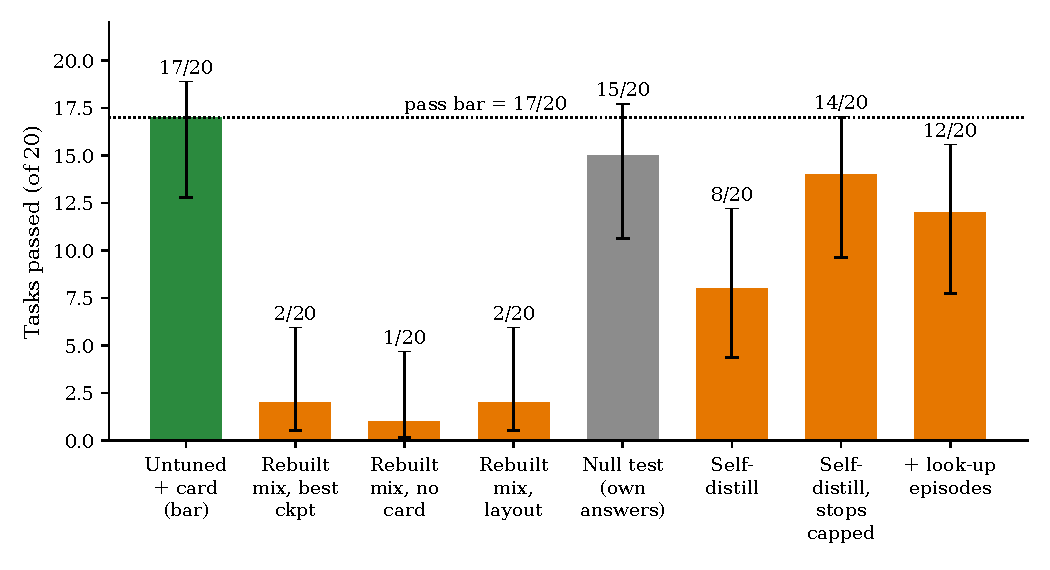
\includegraphics[width=\textwidth]{gate20.pdf}
\caption[Scores on the 20-task gate]{20-task gate (the same 20 tasks for every bar; these are not 200-task accuracies). Error bars: Wilson 95\% intervals, in tasks. Green: the untuned model with the status card, which sets the bar (17/20). Orange: fine-tuned models, run with the card except the one marked ``no card''. Grey: the null test. ``Layout'': continued training on tool lists laid out like the test; ``stops cap'' and ``look-ups'': retrains with the stop share capped or look-up episodes added. Every model trained on the rebuilt mix fails (1--2/20), while the null test stays close to the bar. Self-distillation (training on the model's own checker-approved answers to simulated tasks) and its two rebalanced retrains land in between.}
\label{fig:gate}
\end{figure}


Fine-tuning changed the weights and did not beat the untuned model. The next chapter asks what that means for someone choosing a method.


\chapter{Discussion}
\label{sec:discussion}


\section{State, Not Syntax}

Across these conditions, the hard part is choosing the next step from the current state of the world, including whether to stop. Writing a valid call is the easy part. The levers that help are the ones that support that decision: a summary of real results, a gated stop, and a card that mainly controls whether the model acts. The state summary was meant to put lost facts back in view. What falls, instead, is the number of empty turns. None of the levers reduces state mismatches, and those remain the largest failure type, so the gains come from calling or stopping at the right moment. Tracking the state of the world is still unsolved. Levers that constrain the written form hurt, and training appeared to shift the balance between acting and stopping rather than to improve that tracking.


\section{What We Recommend}

For an on-device agent, use JSON text, a harness-written state summary, a gated stop rule, and a status card. All four are greedy and need no training data or training compute. The minimal recipe, which leaves out the state summary, is a smaller fallback. Writing the same tool list more compactly is a cheap addition: it helped across two paired runs, and it cut context per request by about 30\%. Before any fine-tune, screen on task-level checks rather than validation loss. Even the best run finishes fewer than half of the tasks, and a repeat of the same harness does not pass the same tasks every time. On this benchmark, this model is not yet a reliable multi-step agent.


\section{Limitations}

\begin{itemize}\setlength{\itemsep}{1pt}
  \item \textbf{One model, one split, one device.} All multi-turn results use Gemma-4-E2B-it on the 200-task base split, on one laptop. The stop threshold, the card's fields, and the training filters were chosen on these same tasks. Other models, and the harder splits of the benchmark, are untested.
  \item \textbf{The harness was assembled on these tasks.} The full stack was put together after earlier results on the same 200 tasks were already known, and the family of eight tests was fixed after that. Its gain over JSON text does not survive that correction.
  \item \textbf{Runs move.} Repeating the same harness does not mark the same tasks correct every time. The shorter tool list was tested as two pairs on these same 200 tasks.
  \item \textbf{The screening gate was built from the same split.} The 20 gate tasks were picked using earlier per-task results from the same split, and the bar is the score of the setup the gate is screening. It is a screening check, not a confirmation.
\end{itemize}

The result is the same across the checks in this thesis. The model fails when it must decide the next step, the harness helps that decision, and forcing valid syntax or fine-tuning does not.



\chapter{Future Work and Conclusion}
\label{sec:conclusion}

\section{Future Work}

First, \emph{confirmatory runs}: re-score the full stack and the JSON baseline on held-out tasks, the harder BFCL multi-turn splits and a second small model, with matched serving. Second, \emph{retrieval-augmented tool selection}: retrieve the few relevant tools for each step instead of placing every schema in context~\cite{patil2023gorilla,qin2023toolllm}. The shorter list still sends every tool; it is not this selection step. Third, \emph{decision-balanced training data}: vary the look-up and stop shares with everything else fixed.

\section{Conclusion}

A small model can carry out one tool call and still fail when the task needs a chain of them. The failure is in deciding the next step from the current state of the world, including whether to call, ask, stop, or refuse. Writing a call that only has to parse is the easy part, and forcing every call into valid syntax made the chain worse.

What helped was the harness, the program around the model, with the weights left as they were. It records the current state, stops repeated calls, and shows a short card that advises the next move. That combination raised accuracy by a suggestive amount, and it kept up with a five-sample vote at a fraction of the generation time. Writing the same tool list more compactly helped further. Wrong final states remain the largest failure type. Fine-tuning did not help: the best tuned model scored below the untuned model. For a local agent, these harness changes are also far cheaper than voting or training.


%======================== BACK MATTER ========================
\clearpage
\phantomsection
\tocline{References}
\renewcommand{\bibname}{\textbf{REFERENCES}}
\begingroup
\titleformat{name=\chapter,numberless}[block]{\normalfont\normalsize\bfseries\centering}{}{0pt}{}
\bibliographystyle{unsrtnat}
\bibliography{../paper/references}
\endgroup

\appendix
\clearpage
\addtocontents{toc}{\protect\noindent Appendix\protect\par}
\addtocontents{toc}{\protect\setcounter{tocdepth}{0}}% list appendix titles only
\addtocontents{toc}{\protect\renewcommand{\protect\cftchapaftersnum}{.}}
\renewcommand{\chaptertitlename}{Appendix}

\chapter{Intervention Details}
\label{app:method}

\section{Calls Written as JSON Text}

Following Appendix~B of~\cite{taheri2026iffc}, the tool list is omitted from the API request; the system prompt asks for a JSON list of \texttt{\{function\_name, parameters\}} objects in assistant text. Tool results return as user messages. Calls map to the same BFCL function strings as native calling.

\section{The State Summary Block}

After each successful tool execution, the harness writes a compact \texttt{[STATE]} block from real results (current directory, known files, last executed calls). The last two turns stay verbatim; older raw outputs are dropped. It is not a model-written summary. An example is in Chapter~\ref{sec:setup}.

\section{The Stop Rule}

After a tool result: (1) if the proposed call set equals the previous one, stop; (2) else if every proposed call was already executed in this user request \emph{and} at least six non-empty tool steps have occurred in it, stop; (3) otherwise execute. The six-step window resets on a new user request. The ungated variant applies rule (2) with no minimum.

\section{The Status Card}

Prefixed to a working copy of the latest user message (the stored transcript is unchanged), stacked on stop on repeats. Fields: \texttt{goal} (latest user question, truncated); \texttt{slots} (up to eight key--value facts from executed arguments and results); \texttt{last} (last executed call and outcome); \texttt{next} (advisory: \texttt{refuse} if no tools are available, \texttt{ask} if the last result signals a missing or invalid argument, \texttt{final} if the user's message is a closing ``thanks/done'', otherwise \texttt{call}). The hint does not constrain decoding and the card never reads reference trajectories. It is not the multi-pass OODA-Tool of~\cite{guo2026ooda}. An example is in Chapter~\ref{sec:setup}.

\section{Combining the Full Stack}

The state summary, stop on repeats and status card together: the summary is written into the stored transcript after each executed call, and the card is prefixed to a working copy of the latest user message, as above.

\section{Sampling Five Calls}

On the state-summary configuration, each step samples five completions at temperature 0.7, majority-votes the \texttt{(function\_name, arguments)} tuple, executes the winner once, and continues. It is not a learned verifier.

\section{Two-Pass Constrained Decoding}

Two requests per call: the first constrained to an empty list or a list of valid tool names, the second constraining arguments with each tool's JSON schema. No native tool grammar is active. This approximates XGrammar-2's tag-triggered dispatch~\cite{dong2026xgrammar2} on stock llama-server.

\section{The Tool-Name Automaton}

A live finite automaton restricts the tool name to valid names while arguments are free, on JSON text, not stacked on stop on repeats. Execution accuracy here is not comparable to the F1 reported by Yu et al.~\cite{yu2026ptc}.

\section{Fine-Tuning Setup}

LoRA adapters~\cite{hu2021lora} on Gemma-4-E2B-it with mlx-lm; best-validation checkpoint fused and quantized to Q4\_K\_M; evaluated with JSON text. The rebuilt mix: 30{,}000 training / 1{,}500 validation rows; 45/40/10/5\% simulated / APIGen / ToolACE / xLAM; 22\% empty-list targets (all after a tool result); 41.2\% of rows with multi-call targets; no evaluation tool names copied into simulations. DPO: $\beta{=}0.2$, LoRA, scored on JSON text.

\chapter{Failure Labels, Exploratory Tests and Training History}
\label{app:fail}

\begin{table}[H]
\centering
\footnotesize
\setlength{\tabcolsep}{3pt}
\caption[Primary error for each failed task]{Primary error per failed task (200 tasks). Native is the native API. JSON text is calls written as JSON text. Stop = stop on repeats (gated); Ungated = stop on first repeat; Summary = state summary; Minimal = minimal recipe; Full = full stack; Vote = vote of five; CD = constrained decoding; Autom.\ = tool-name automaton; SFT = best fine-tune. Labels as defined in Chapter~\ref{sec:setup}.}
\label{tab:failfull}
\begin{tabular}{@{}lrrrrrrrrrrr@{}}
\toprule
Label & Native & JSON text & Stop & Ungated & Summary & Minimal & Full & Vote & CD & Autom. & SFT \\
\midrule
Empty turn & 59 & 41 & 38 & 40 & 31 & 17 & 20 & 36 & 14 & 17 & 2 \\
Under-call & 19 & 38 & 37 & 31 & 37 & 41 & 35 & 38 & 70 & 54 & 59 \\
State mismatch & 68 & 60 & 60 & 75 & 64 & 71 & 68 & 53 & 95 & 102 & 109 \\
\midrule
Failed & 146 & 139 & 135 & 146 & 132 & 129 & 123 & 127 & 179 & 173 & 170 \\
\bottomrule
\end{tabular}
\end{table}

\begin{table}[H]
\centering
\footnotesize
\caption[Exploratory paired tests]{Exploratory McNemar tests, outside the eight-test correction family (uncorrected $p$; columns as in Table~\ref{tab:mcnemar}).}
\label{tab:mcnemar-x}
\begin{tabular}{@{}llrrr@{}}
\toprule
A & B & A only & B only & $p$ \\
\midrule
State summary (34.0\%) & JSON text (30.5\%) & 20 & 13 & 0.30 \\
Vote of five (36.5\%) & State summary & 17 & 12 & 0.46 \\
Stop on repeats (32.5\%) & JSON text & 11 & 7 & 0.48 \\
Minimal recipe (35.5\%) & Stop on repeats & 26 & 20 & 0.46 \\
\bottomrule
\end{tabular}
\end{table}

\section{Training History}
\label{app:train}

\subsection{Version History}

Dropping only mid-dialogue empty targets from the first mix still scored 1/200; deleting trailing empty answers at serving time scored 4/200. After the repaired mix (30/200), two further filtering variants scored 23/200 and 26/200 (Table~\ref{tab:board}); each changed several filters at once, so they are not single-factor ablations. The rebuilt mix's training was stopped early at step 26{,}500 of 32{,}000; the best validation loss (0.030) was at step 22{,}000, and that checkpoint is the one evaluated. Continued training for 2{,}500 steps on tool lists laid out like the test scored 2/20.

\subsection{A Candidate Cause That Targeted Retrains Did Not Confirm}

\emph{Self-distillation} (training on the model's own answers to simulated tasks, keeping only turns the task checker marked correct) scored 8/20; in 6 of 12 failures the model said an ID or price was missing and stopped instead of calling the tool that would supply it. Compared with the null-test data, look-up-type calls (a name-matching heuristic) fell from 37.9\% to 19.7\% of calls and stop targets rose from 23.1\% to 33.2\%. Two targeted retrains tested this: capping the stop share scored 14/20, and restoring the look-up share (39.6\%) scored 12/20. Neither passed, so the data are \emph{consistent with}, but do not establish, a shift in the decision mix (stop versus continue, look up versus act) as the cause. Leak checks found no evaluation task IDs or tool names in the null-test or self-distillation data.

\subsection{Self-Distillation Counts}

Look-up-type calls: 67/177 in the null-test data versus 78/395 in the self-distillation data; stop targets: 36/156 versus 146/440. Capping the stop share (22.9\%) left the look-up share low (20.6\%). The look-up-restoring retrain lost 7 tasks the untuned model solves, and empty turns returned (9 of 66 turns). Look-up counts rest on a name-matching heuristic.

\subsection{Stop Targets in the Rebuilt Mix}

Stop targets were 22\% of all rebuilt-mix rows, all after a tool result, a different denominator from the first mix's 78.1\% (the share of targets \emph{after a tool result} that were stops). The rebuilt-mix models still under-called, so stop share alone does not explain the collapse.



\chapter{Full Scoreboard and Reproducibility}
\label{app:runs}

\begin{table}[H]
\renewcommand{\arraystretch}{1.0}
\centering
\setlength{\tabcolsep}{3pt}
\caption[Every scored condition]{Every scored condition (Gemma-4-E2B-it Q4\_K\_M). The ID is the internal log id, with the internal name in parentheses. Interval: Wilson 95\%. Rows of 20 are screening checks, not 200-task accuracies.}
\label{tab:board}\label{tab:runs}
\scriptsize
\setlength{\aboverulesep}{0.5pt}
\setlength{\belowrulesep}{0.5pt}
\begin{tabular}{@{}r>{\RaggedRight\arraybackslash}p{9.0cm}rrl@{}}
\toprule
ID & Condition & Result & Acc. & 95\% interval \\
\midrule
\multicolumn{5}{@{}l}{\emph{Multi-turn base, 200 tasks}} \\
84 & Shorter tool list on the full stack, second pair (best single run)$^{a}$ & 88/200 & 44.0\% & 37.3--50.9 \\
83 & Shorter tool list on the full stack, first pair$^{a}$ & 84/200 & 42.0\% & 35.4--48.9 \\
78 & Full stack, first run (\texttt{iffc-state-ooda}, PR \#90) & 77/200 & 38.5\% & 32.0--45.4 \\
11 & Vote of five on state summary (BoN $N{=}5$ on IFFC+STATE) & 73/200 & 36.5\% & 30.1--43.4 \\
85 & Full stack, second rerun, original tool list$^{a}$ & 72/200 & 36.0\% & 29.7--42.9 \\
82 & Full stack, fresh rerun, original tool list$^{a}$ & 71/200 & 35.5\% & 29.2--42.3 \\
42 & Minimal recipe: card on stop on repeats (``R42'') & 71/200 & 35.5\% & 29.2--42.3 \\
10 & State summary (IFFC+STATE) & 68/200 & 34.0\% & 27.8--40.8 \\
30 & Stop on repeats, gated at six steps (MIN=6) & 65/200 & 32.5\% & 26.4--39.3 \\
5 & JSON text (IFFC) & 61/200 & 30.5\% & 24.5--37.2 \\
9 & Guided template on native API (GST+NFC) & 61/200 & 30.5\% & 24.5--37.2 \\
4 & Native API (NFC) & 54/200 & 27.0\% & 21.3--33.5 \\
27 & Stop on first repeat (ungated) & 54/200 & 27.0\% & 21.3--33.5 \\
51 & DPO, full train & 53/200 & 26.5\% & 20.9--33.0 \\
15 & Best SFT, repaired mix (SFT-v4) & 30/200 & 15.0\% & 10.7--20.6 \\
46 & Tool-name automaton (PTC-A) & 27/200 & 13.5\% & 9.4--18.9 \\
18 & SFT, filters on first-turn targets off$^\dagger$ (SFT-v6) & 26/200 & 13.0\% & 9.0--18.4 \\
16 & Best SFT + state summary (SFT-v4+STATE) & 26/200 & 13.0\% & 9.0--18.4 \\
17 & SFT, extra first-turn and state filters$^\dagger$ (SFT-v5) & 23/200 & 11.5\% & 7.8--16.7 \\
8 & Constrained decoding, two-pass (CD) & 21/200 & 10.5\% & 7.0--15.5 \\
14 & SFT first mix, trailing empty answers stripped (SFT-v2 strip) & 4/200 & 2.0\% & 0.8--5.0 \\
12, 13 & SFT first mixes, two variants (SFT-v1, SFT-v2) & 1/200 each & 0.5\% & 0.1--2.8 \\
\multicolumn{5}{@{}l}{\emph{20-task gate (same 20 tasks for every row)}} \\
69 & Untuned + card: gate bar & 17/20 & & \\
70 & Rebuilt mix, best-validation checkpoint (SFT-v11, step 22{,}000) & 2/20 & & \\
71 & Rebuilt mix, no card & 1/20 & & \\
72 & Rebuilt mix, layout continue-train (SFT-v11 fmt2500) & 2/20 & & \\
73 & Null test (v13 null) & 15/20 & & \\
74 & Self-distillation, correct turns only (v13-sd) & 8/20 & & \\
75 & Self-distillation, stop share capped (v13-sdb) & 14/20 & & \\
76 & Self-distillation + simulated look-up episodes (v13-lk) & 12/20 & & \\
\multicolumn{5}{@{}l}{\emph{Single-call BFCL v4 categories, native API$^\ddagger$}} \\
79 & Three categories below (weighted) & 772/840 & 91.9\% & 89.9--93.6 \\
 & \quad Simple (one function offered) & 375/400 & 93.75\% & \\
 & \quad Multiple (several functions; pick the right one) & 183/200 & 91.50\% & \\
 & \quad Irrelevance (no call needed) & 214/240 & 89.17\% & \\
\bottomrule
\end{tabular}

\parbox{\linewidth}{\RaggedRight\scriptsize $^\dagger$First-turn filters drop or require training examples where the first response is empty or under-specified; state filters drop continuations inconsistent with executed tool results. $^\ddagger$The two parallel-call categories are excluded because earlier runs on this server hit a tool-grammar bug that truncated multi-call output. $^{a}$Run 80 (scores.id 59) is the 10-task original list, 5/10. Run 81 (scores.id 60) is the 10-task shorter list, 8/10. Recorded calls differed from the first full-stack run on tasks 55, 69, 26, 179, and 59. The plan's gate required 0 of 10 to differ, so the gate failed. Run 82 is the 200-task original list and run 83 the 200-task shorter list (pair 1, $p=0.053$). Runs 84 (shorter list, run first) and 85 (original list) are pair 2 ($p=0.011$). Across both pairs the shorter list does better on 33 tasks and worse on 17 (sign test, $p=0.033$).}
\end{table}

\begin{sloppypar}
\section{Reproducibility}

Hardware: MacBook Pro, Apple M4~Pro, 48~GB, with Metal acceleration (Apple's GPU interface). Earlier runs in this thesis are recorded as llama.cpp build 8111 (commit \texttt{11c325c6e}). Runs 78 and 80--85 used commit \texttt{d344123fe}, with \texttt{llama-server -{}-jinja -fa on -ngl 99 -c 65536 -{}-temp 0.0 -np 4 -cb -ub 1024}. The native-API baseline used \texttt{-np 8}. BFCL v4 via the \texttt{bfcl-eval} package (exact version per run not logged). Temperature 0 except voting (0.7, $N{=}5$, one seed). The full stack (ID 78 in Table~\ref{tab:board}) is \texttt{benchmark.db} \texttt{scores.id} 51 with log \path{sft/v13/paper_evals/runs/b_fullstack_mtb200.log}; its harness code is pull request \#90, run at commit \texttt{344ce45} and merged as \texttt{83f35ee}. The shorter-list runs are 80 (scores.id 59, 10-task original list, log \path{R81_slim/smoke_off.log}), 81 (scores.id 60, 10-task shorter list, \path{R81_slim/smoke_on.log}), 82 (scores.id 61, 200-task original list, \path{R81_slim/full_off.log}), and 83 (scores.id 62, 200-task shorter list, \path{R81_slim/full_on.log}). The second pair is runs 84 (scores.id 63, 200-task shorter list, \path{R82_confirm/full_on.log}) and 85 (scores.id 64, 200-task original list, \path{R82_confirm/full_off.log}). Opening-prompt lengths are medians from \path{R81_slim/*.metrics.jsonl}. Failure labels for the other rows are derived from the checker messages in the \texttt{eval\_errors} table. Figures are regenerated from these counts by \texttt{paper/\allowbreak{}figures/\allowbreak{}src/\allowbreak{}make\_refocus\_figs.py}. Single-call ID 79 is the simple, multiple, and irrelevance rows in the log \path{sft/v13/paper_evals/runs/a_single_turn_gemma.log}; the 91.9\% interval is that script's Wilson formula on 772/840.
\end{sloppypar}

\section{Shorter Tool List Checks}
\label{app:trim}

A 10-task check scored 5 of 10 with the original list and 8 of 10 with the shorter list. The recorded calls differed from the first full-stack run on five tasks. The plan required none of those ten to differ, so that check failed. The plan had paired the test with the first full-stack run (77 of 200). After the check failed, the comparison used a fresh rerun of the original list instead.

The context window is 16{,}384 tokens per request (65{,}536 shared across four slots). The opening prompt on the original list is about 5{,}000 tokens. Its median length falls from 4{,}923.5 tokens to 2{,}888, a 41\% cut (41.3\%). Mean context per request falls from 7{,}107 tokens to 4{,}990, about 30\%. Invalid tool names stay at zero (0 of 1{,}276 calls with the shorter list, 0 of 1{,}244 with the original list). Invalid arguments are 2 of 1{,}276 against 9 of 1{,}244. Format errors are 1 of 1{,}801 model replies against 0 of 1{,}773. Mean server time per model request, prompt reading plus generation, with four slots, is 15.4\,s with the shorter list and 18.8\,s with the original list (medians 12.7\,s and 15.9\,s). Most of the drop is generation (16.2\,s to 13.5\,s). Prompt reading falls from 2.53\,s to 1.86\,s.

The second pair shows the same pattern. Mean context per request falls from 7{,}121 tokens to 5{,}001, again about 30\%, and mean server time per request from 19.4\,s to 15.4\,s, about 20\% faster. Invalid tool names and format errors are zero for both lists. Invalid arguments are 4 of 1{,}300 calls with the shorter list against 5 of 1{,}255 (0.31\% and 0.40\%).


\end{document}
